\documentclass[a4paper,11pt,titlepage]{article}

\usepackage{latexsym}
\usepackage{graphicx}
\usepackage{float}
\usepackage{url}
\usepackage{unicode}
\usepackage[polish]{babel}
\usepackage{titlesec}
\usepackage{listings}
\usepackage{xcolor}
\usepackage{setspace}
\usepackage{subfig}
\usepackage{tabularx}
\usepackage{courier}
\DeclareUnicodeCharacter{200B}{{\hskip 0pt}}

\definecolor{codeblue}{rgb}{0,0,0.6}
\definecolor{codegray}{rgb}{0.5,0.5,0.5}
\definecolor{codepurple}{rgb}{0.58,0,0.82}
\definecolor{backcolour}{rgb}{0.96,0.96,0.96}

\lstdefinestyle{code}{
    backgroundcolor=\color{backcolour},
    keywordstyle=\color{codeblue},
    numberstyle=\tiny\color{codegray},
    stringstyle=\color{codeblue},
    basicstyle=\ttfamily\footnotesize,
    breakatwhitespace=false,
    breaklines=true,
    captionpos=b,
    keepspaces=true,
    numbers=left,
    numbersep=3pt,
    showspaces=false,
    showstringspaces=false,
    showtabs=false,
    tabsize=1,
    basicstyle=\small
}

\lstset{style=code}

\newcommand{\sectionbreak}{\clearpage}
\author{Adam Talarczyk}
\title{Symulacja Wieloagentowa}
\frenchspacing
\begin{document}
\begin{titlepage}
    \begin{center}

        \Huge
        \textbf{WYDZIAŁ NAUK ŚCISŁYCH I TECHNICZNYCH}
        
        
        \vspace{1.5cm}
	   Symulacje Komputerowe
        \LARGE
        
	\vspace{2cm}
	
	Sprawozdanie ``Symulacja Wieloagentowa''

	\vspace{1cm}
	Adam Talarczyk, Mateusz Wrzoł
	
	\vspace{5cm}
        \vfill

        \vspace{0.8cm}
	\Large
        Uniwersytet Śląski, Sosnowiec, 2021

    \end{center}
\end{titlepage}
\newpage

\tableofcontents
\newpage

\section{Zadanie 1}
Należy opracować symulator dowolnego zjawiska lub procesu, wykorzystując model wieloagentowy.

Symulator powinien być wyposażony następujące funkcje:
\begin{itemize}
\item wizualizacja stanu środowiska i agentów,
\item wykres(y) z wynikami symulacji,
\item interfejs użytkownika umożliwiający modyfikowanie parametrów modelu.
\end{itemize}


Sprawozdanie powinno zawierać:
\begin{itemize}
\item opis zaimplementowanego modelu wieloagentowego,
\item kod źródłowy symulatora z komentarzami,
\item prezentację interfejsu użytkownika z zrzutami ekranu,
\item przykładowe wyniki symulacji,
\item spis bibliografii (jeżeli była wykorzystana).
\end{itemize}

Dodatkowo poza sprawozdaniem proszę przesłać pik(i) z projektem symulatora (np. plik Netlogo).

Ocena rozwiązania będzie uwzględniała:
\begin{itemize}
\item stopień skomplikowania zaproponowanego modelu i opracowanego symulatora,
\item oryginalność rozwiązania (symulator nie może być prostą modyfikacją modeli symulacyjnych dostępnych w Netlogo lub innego gotowego oprogramowania),
\item jakość przygotowanego sprawozdania.
\end{itemize}

Do rozwiązania zadania można wykorzystać środowisko Netlogo lub dowolne inne środowisko programistyczne.

%Symulacja
\section{Symulacja środowiska ptaszników}
Wykonana w sprawozdaniu symulacja jest odwzorowaniem naturalnego środiwiska ptaszników z uwzględnieniem ich charakterystycznych zachowań. Ponadto, symulacja pozwala na zmianę wielu czynników wpływając na zachowania symulowanych obiektów.

Rozdział zawiera opis zaimplementowanego modelu wieloagentowego, kod źródłowy z komentarzami oraz prezentację interfejsu użytkownika.

%Opis zaimplementowanego modelu
\subsection{Opis modelu}

%Sources
\subsection{Kod źródłowy symulatora}

%Interfejs
\subsection{Interfejs użytkownika}
Interfejs użytkownika został przedstawiony na rysunku \ref{fig:9}, wyszczególnić można 3 kategorie:
\begin{itemize}
	\item Konfiguracja symulacji i środowiska
	\item Pole na którym wyświetlana jest symulacja
	\item Panel raportowania, zawierający dane i wykresy
\end{itemize}

\begin{figure}[H]
\centering
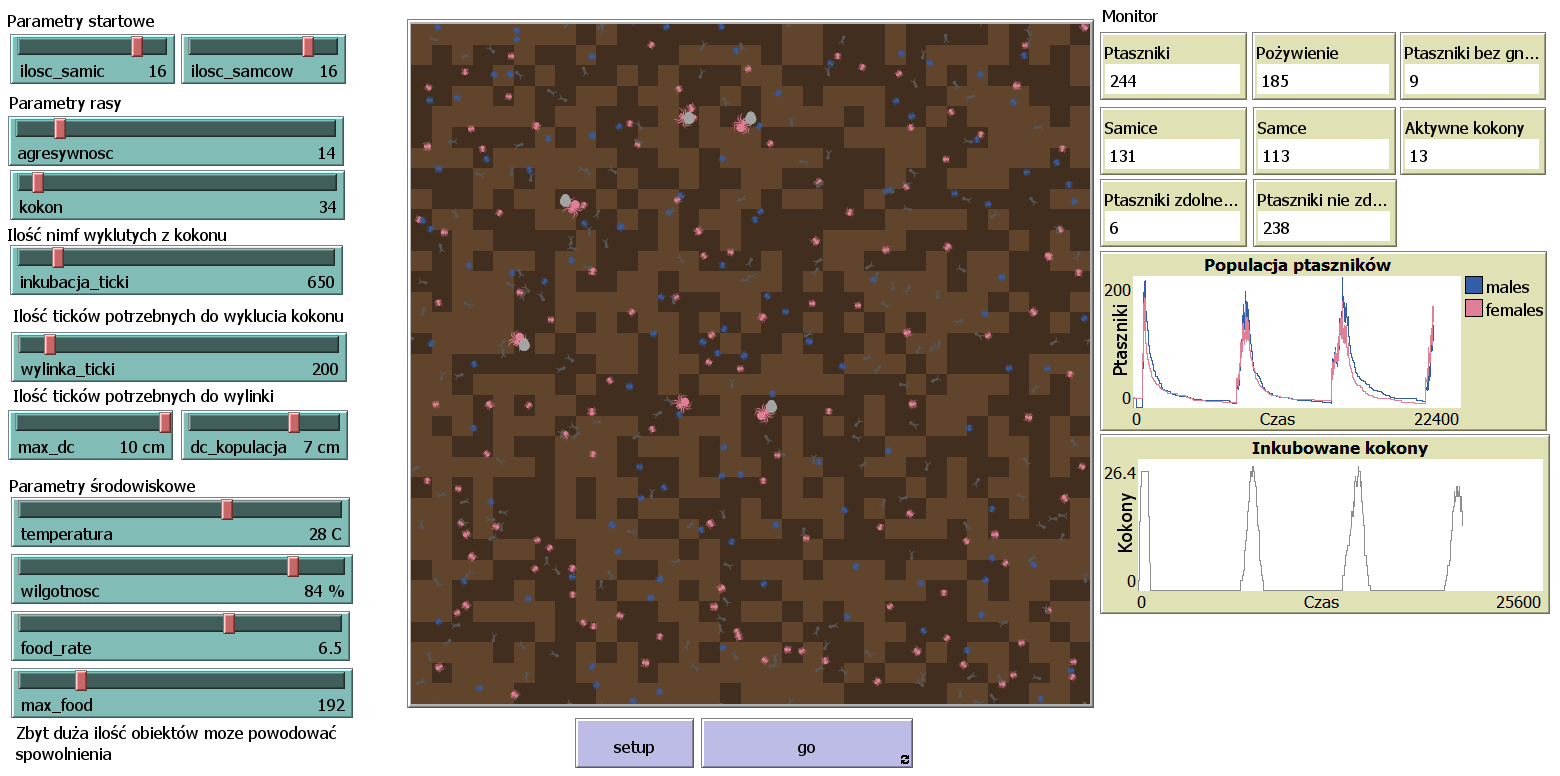
\includegraphics[width=1\columnwidth]{img/symulacja.PNG}
\caption{Obszar symulacji}
\label{fig:9}
\end{figure}

% Opis parametrów i kontrolek
Obszar konfiguracji środowiska również podzielony jest na kategorie. Parametry startowe zaprezentowane na rysunku \ref{fig:6} (tj. \textit{ilosc\_samic}, \textit{ilosc\_samcow}) określają ile dorosłych samic i samców podczas inicjalizacji ma zostać wygenerowanych.

\begin{figure}[H]
\centering
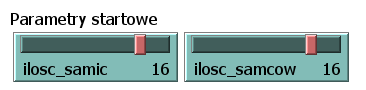
\includegraphics[width=.5\columnwidth]{img/parametry_startowe.PNG}
\caption{Kontrolki odpowiedzialne za parametry startowe}
\label{fig:6}
\end{figure}

Parametry rasy (rysunek \ref{fig:5} określają ogólne zachowanie ptaszników:
\begin{itemize}
\item \textit{agresywnosc} - zachowanie w stosunku do innych ptaszników. Wartość 0 oznacza, że nie będąze sobą w ogóle walczyć, \item wartość 100 – walka przy każdym spotkaniu. 
\item \textit{kokon} - ilość młodych nimf wyklutych z pojedynczego kokonu 
\item \textit{inkubacja\_ticki} - ilość czasu potrzebne do wyinkubowania kokonu
\item \textit{wylinka\_ticki} - ilość czasu, potrzebna do odbycia kolejnej wylinki. Wylinka wiąże się ze wzrostem DC pająka. 
\item \textit{max\_dc} – maksymalny rozmiar, który może osiągnąć ptasznik. 
\item \textit{dc\_kopulacja} – wymagany rozmiar ptasznika aby osiągnąć zdolności kopulacyjne 
\end{itemize}

\begin{figure}[H]
\centering
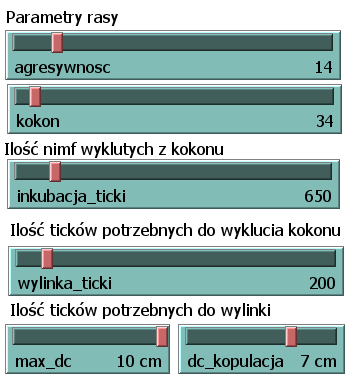
\includegraphics[width=.5\columnwidth]{img/parametry_rasy.PNG}
\caption{Kontrolki odpowiedzialne za parametry rasy}
\label{fig:5}
\end{figure}


Parametry środowiskowe - ogólne parametry odpowiedzialne za środowisko, temperaturę, wilgotność oraz ilość pożywienia na ekranie (rysunek \ref{fig:4}):
\begin{itemize}
\item \textit{temperatura}, \textit{wilgotnosc} - parametry, które mogą być zmieniane podczas symulacji. Stosując wartości skrajne można spowodować zachowania uboczne, np. Umieranie ptaszników, niszczenie kokonów.
\item \textit{food\_rate} - mnożnik jedzenia, im większy, tym więcej pożywienia pojawia się na ekranie.
\item \textit{max\_food} - maksymalna ilość pożywienia na ekranie jednocześnie. Zbyt duża ilość może powodować problemy optymalizacyjne. 
\end{itemize}

\begin{figure}[H]
\centering
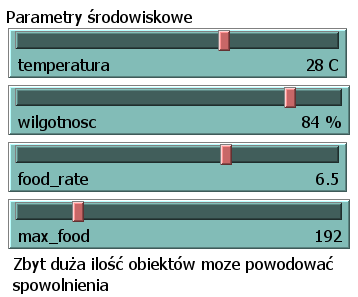
\includegraphics[width=.5\columnwidth]{img/parametry_env.PNG}
\caption{Kontrolki odpowiedzialne za parametry środowiskowe}
\label{fig:4}
\end{figure}

% opis symulacji i ikon
Obszar symulacji zaprezentowano na rysunku \ref{fig:1}. Po obszarze poruszają się ptaszniki, których płeć można rozróżnić przez charakterystyczne kolory. Kolor różowy oznacza samicę, a niebieski samca (rysunek \ref{fig:icons1}). Dodatkowo, na obszarze symulacji wyszczególnić można ikony kokonu i pożywienia (rysunek \ref{fig:icons2}).
\begin{figure}[H]
\centering
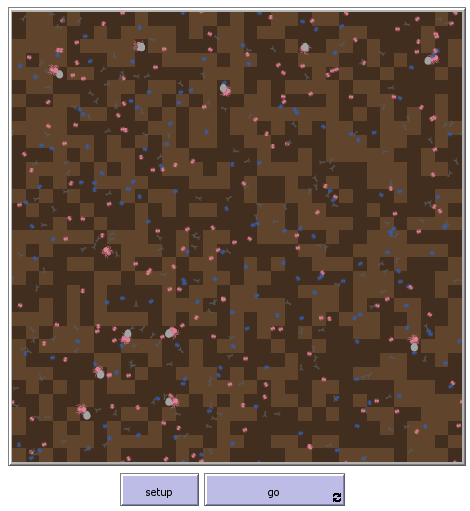
\includegraphics[width=.75\columnwidth]{img/map.PNG}
\caption{Obszar wizualizacji symulacji}
\label{fig:1}
\end{figure}

\begin{figure}[H]%
    \centering
    \subfloat[\centering Ikona samicy]{{
\includegraphics[width=3cm]{img/samica.PNG} }}%
    \qquad
    \subfloat[\centering Ikona samca]{{
\includegraphics[width=3cm]{img/samiec.PNG} }}%
    \caption{Ikony samców i samic w symulacji}%
    \label{fig:icons1}%
\end{figure}

\begin{figure}[H]%
    \centering
    \subfloat[\centering Ikona pokarmu]{{
\includegraphics[width=3cm]{img/bug.PNG} }}%
    \qquad
    \subfloat[\centering Ikona kokonu]{{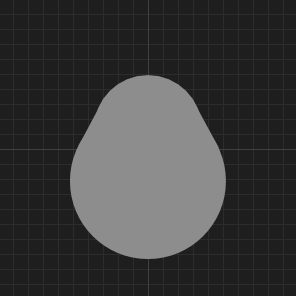
\includegraphics[width=3cm]{img/egg.PNG} }}%
    \caption{Pozostałe ikony użyte w symulacji}%
    \label{fig:icons2}%
\end{figure}

Dodatkowo, środowisko NetLogo pozwala na śledzenie obiektów w czasie rzeczywistym, zaprezentowane zostało to na rysunku \ref{fig:8}

\begin{figure}[H]
\centering
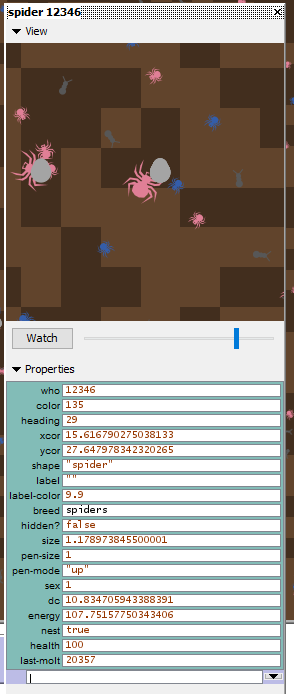
\includegraphics[width=.5\columnwidth]{img/spider-params.PNG}
\caption{Parametry ptasznika w trakcie trwania symulacji.}
\label{fig:8}
\end{figure}


%Opis danych i wykresów
Ostatnim elementem jest prezentacja danych i wyników. Odpowiedzialne jest za to monitor (rysunek \ref{fig:2}). 
\begin{figure}[H]
\centering
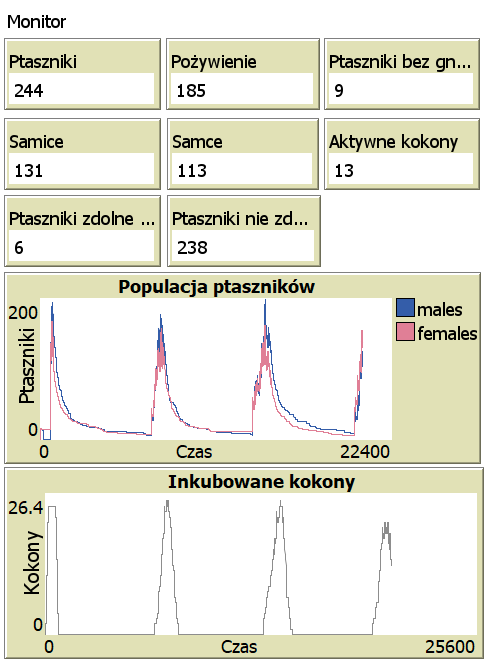
\includegraphics[width=.5\columnwidth]{img/monitor.PNG}
\caption{Monitor - reprezentacja danych symulacji}
\label{fig:2}
\end{figure}

\noindent Monitor podzielony został on na dane i wykresy. Dane przedstawiają sumaryczna ilość ptaszników z podziałem na samce, samice, ptaszniki zdolne i niezdolne do kopulacji. Dodatkowo, wyświetlana jest ilość pożywienia, ilość ptaszników bez gniazda oraz aktywne, inkubowane kokony (rysunek \ref{fig:3}).

\begin{figure}[H]
\centering
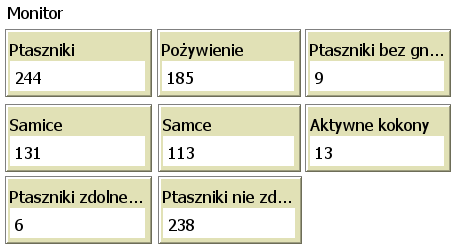
\includegraphics[width=.5\columnwidth]{img/monitor_danych.PNG}
\caption{Poszczególne dane}
\label{fig:3}
\end{figure}

Wykresy przedstawiają w czasie rzeczywistym populację ptaszników z podziałem na samce i samice. Ostatni wykres przedstawia ilość kokonów (rysunek \ref{fig:10}).
\begin{figure}[H]
\centering
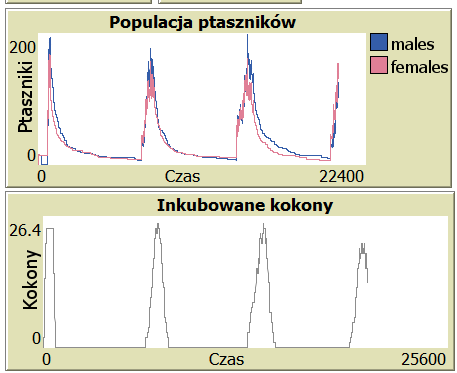
\includegraphics[width=.8\columnwidth]{img/wykresy.PNG}
\caption{Wykresy}
\label{fig:10}
\end{figure}

\subsection{Wyniki symulacji}
Wyniki symulacji przedstawiane są w czesie rzeczywistym na monitorze danych. Wizualna reprezentacja przedstawiona jest na wykresach (rysunek \ref{fig:10}). Zauważyć można zależność, że populacja ptaszników rośnie i maleje co jakiś interwał. Wynika to z charakterystyki ich zachowania, samce żyją znacznie krócej od samic i umierają niedługo po wylince umożliwiającej im kopulację. Ilość ptaszników, które przeżywa zależna jest od ilości pożywienia, agresywności rasy i innych przypadkowych czynników. Podsumowując, tylko niewielka ilość ptaszników dożywa momentu, w którym jest zdolna do kopulacji. Mimo to, w symulacji występuje ciągłość- gatunek nie wymiera przy optymalnych parametrach.

\newpage
\addcontentsline{toc}{section}{Spis rysunków}
\listoffigures
\newpage

\addcontentsline{toc}{section}{Tabele}
\listoftables

\begin{thebibliography}{5}
\addcontentsline{toc}{section}{Bibliografia}
\bibitem{1}
https://ccl.northwestern.edu/netlogo/docs/programming.html
\bibitem{2}
https://ccl.northwestern.edu/netlogo/docs/dictionary.html

\end{thebibliography}


\end{document}
